\chapter{The hexagonal extension}\label{ch:hexagonal}

The handbook's extension 7 replaces the rectangular lattice by a hexagonal one
\cite{handbook2020}. The model has a few quantities that are supposed to be universal
and many that are not, and a change of lattice separates them. This chapter defines the
extension, shows that it inherits the Abelian property rather than needing a new proof,
and compares it with the square baseline quantity by quantity.

\section{Model: a hexagonal lattice}\label{sec:hexmodel}

Sites are indexed by axial coordinates $\bm{x} = (q,r) \in \mathbb{Z}^2$, with six
neighbour directions
\begin{equation}\label{eq:hexdirs}
  (1,0),\ (0,1),\ (-1,1) \quad\text{and their opposites} \quad
  (-1,0),\ (0,-1),\ (1,-1) .
\end{equation}
Each site therefore has exactly six neighbours, and the tiling whose cells are centred
on the sites is the hexagonal one: the cells are regular hexagons and the lattice of
cell centres is triangular. The region is a hexagon of radius $R$,
\begin{equation}\label{eq:hexregion}
  \bm{L}_{\hx} = \{(q,r) : \max(\abs{q}, \abs{r}, \abs{q+r}) \le R\},
  \qquad
  N_{\hx} = \abs{\bm{L}_{\hx}} = 3R^2 + 3R + 1 ,
\end{equation}
chosen because its boundary is a single closed ring at constant graph distance $R$ from
the centre. There are no $90^\circ$ corners: the boundary turns through $120^\circ$ six
times.

Two different objects are called ``hexagonal''. The honeycomb graph --- graphene, the
hexagonal \emph{tiling} --- has three edges per vertex; the lattice used here is the
triangular lattice, whose \emph{cells} are hexagons, with six. The model is the
six-neighbour one, as the handbook intends, and the distinction matters below: the
threshold is fixed by the number of neighbours, so the honeycomb graph would force
$k = 3$.

\begin{figure}[htbp]
\begin{center}
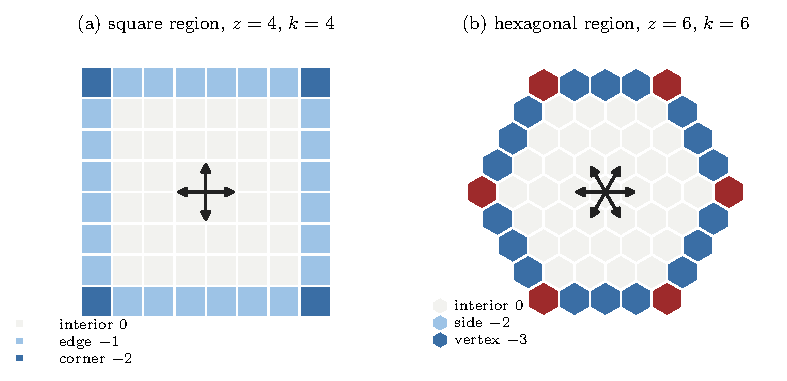
\includegraphics[width=0.70\linewidth]{figures/lattice.pdf}
\end{center}
\caption{The two lattices, coloured by the row sum of the toppling matrix, which is the
loss incurred by one toppling at that site. Left: the square region, with $0$
(interior), $-1$ (edge) and $-2$ (corner). Right: the hexagonal region, with $0$
(interior), $-2$ (side) and $-3$ (vertex). The regions are drawn at matched size ---
$N = 64$ and $N = 61$ --- so that the boundary classes compare directly; the arrows
mark the four and six toppling directions.}
\label{fig:lattice}
\end{figure}

\section{The threshold is locked by conservation}\label{sec:hextheta}

The toppling matrix is the direct analogue of \eqref{eq:delta}:
\begin{equation}\label{eq:deltah}
  \Dhex(\bm{x},\bm{y}) =
  \begin{cases}
    -6, & \bm{x} = \bm{y}, \\
    \phantom{-}1, & \bm{y} - \bm{x} \in \text{\eqref{eq:hexdirs}}, \\
    \phantom{-}0, & \text{otherwise}.
  \end{cases}
\end{equation}
The four conditions are checked as before, and the check is short enough to write out,
because it is where the threshold is decided. \emph{\eqref{eq:4a}}: the direction set
\eqref{eq:hexdirs} is closed under negation, so the neighbour relation is symmetric and
the off-diagonal entries are all $+1 \ge 0$. \emph{\eqref{eq:4b}}: the diagonal is
$-6 < 0$, so
\begin{equation}\label{eq:khex}
  k_{\hx} = -\Dhex(\bm{x},\bm{x}) = 6 .
\end{equation}
\emph{\eqref{eq:4c}}: with $m(\bm{x})$ the number of the six neighbours lying inside
$\bm{L}_{\hx}$,
\begin{equation}\label{eq:rowsumhex}
  \sum_{\bm{y}} \Dhex(\bm{x},\bm{y}) = -6 + m(\bm{x}) \le 0 ,
\end{equation}
with equality for interior sites and strict inequality at the boundary.
\emph{\eqref{eq:4d}}: the region is finite with a boundary, so the total
$\sum_{\bm{x}}(-6 + m(\bm{x})) = -12R-6$ is negative.

The threshold is therefore not a second modelling choice; it is what the matrix says. If
the threshold were left at $4$ while six grains are sent out, an interior toppling would
have row sum $+2$: each toppling would \emph{create} two grains, condition \eqref{eq:4c}
would fail, the total mass would grow without bound, and by
Proposition~\ref{prop:termination} there would be no reason for an avalanche to stop.
Conversely, keeping $k=4$ by sending grains to only four of the six neighbours would make
the neighbour relation asymmetric, so $\Dhex$ would no longer be a graph Laplacian. There
is no way to change the degree without changing the threshold.

What that does to the loss is visible in the row sums (Table~\ref{tab:rowsums}).

\begin{table}[htbp]
\centering
\small
\caption{Row-sum classes of $\D$ on the two lattices. The hexagonal classes are
$\{0,-2,-3\}$: the value $-1$ does not occur, and the deepest class is one grain deeper
than on the square lattice.}
\label{tab:rowsums}
\begin{tabular}{llrr}
\toprule
\textbf{Lattice} & \textbf{Class} & \textbf{Row sum} & \textbf{Number of sites} \\
\midrule
\multirow{3}{*}{square $L \times L$}
  & interior & $0$  & $(L-2)^2$ \\
  & edge     & $-1$ & $4(L-2)$  \\
  & corner   & $-2$ & $4$       \\[2pt]
\multirow{3}{*}{hexagon radius $R$}
  & interior & $0$  & $3R^2-3R+1$ \\
  & side     & $-2$ & $6(R-1)$    \\
  & vertex   & $-3$ & $6$         \\
\bottomrule
\end{tabular}
\end{table}

Three features of the table matter later. First, the hexagon has three loss classes like
the square, but a different three: $\{0,-2,-3\}$ rather than $\{0,-1,-2\}$, since every
non-interior site of a hexagonal region has either two or three of its six neighbours
outside, so that the transition from interior to boundary is a jump of two grains rather
than one. Second, the deepest class is deeper: a hexagon vertex has three directions off
the board, against two for a square corner, so there are six points of strongest
dissipation rather than four and each of them loses more per toppling. Third, the
deepest class carries a larger share of the total loss. The dissipation capacity
$\sum_{\bm{x}}(-\text{row sum})$ is $4L$ on the square and $12R+6$ on the hexagon, of
which the deepest class accounts for $8$ and $18$; at equal $N$ these become
$2/\sqrt{N}$ against $3\sqrt{3}/(2\sqrt{N})$, larger by a factor
$3\sqrt{3}/4 \approx 1.30$ (Figure~\ref{fig:scaling}c). What is narrower on the hexagon
is the relative spread within the boundary: per toppling a square boundary site loses $1$
or $2$ grains, a factor $2$, against $2$ or $3$, a factor $1.5$.

\section{The metric has to change with the geometry}\label{sec:hexmetric}

On the square lattice the graph distance is the Manhattan distance, which is why
\eqref{eq:manhattan} is the right definition of $R$: $R$ counts steps. On the hexagonal
lattice the shortest path along the six directions is
\begin{equation}\label{eq:hexdist}
  d_{\hx}(\bm{x},\bm{y}) =
  \max\bigl(\abs{\Delta q},\ \abs{\Delta r},\ \abs{\Delta q + \Delta r}\bigr),
  \qquad \Delta q = q_{\bm{y}} - q_{\bm{x}},\ \ \Delta r = r_{\bm{y}} - r_{\bm{x}} ,
\end{equation}
and the length observable must be redefined as
$R_{\hx} = \max_{\bm{y}:\,\sigma(\bm{y}) > 0} d_{\hx}(\bm{x}_0, \bm{y})$.

Keeping the Manhattan distance would be a silent error, and a large one: two sites at
hexagonal distance $d$ have axial $L^1$ distance between $d$ and $2d$, since a straight
run in one direction and a diagonal run of the same hexagonal length are equally far in
the graph metric but differ by a factor of two in $L^1$. Using $L^1$ would inflate
measured lengths by up to a factor of two depending on the avalanche's direction, and
the threshold relation between $l$ and $R$ of §\ref{sec:correlations} would be lost
while the rest of the code continued to run.

The metric also changes the counting of sites within a radius, which affects finite-size
scaling even in a correct implementation. A ball of graph radius $R$ holds
$2R^2+2R+1$ sites on the square lattice and $3R^2+3R+1$ on the hexagonal one, a ratio
approaching $3/2$ (Figure~\ref{fig:scaling}a), so an avalanche of a given radius can
involve half again as many sites; and at equal $N$ the hexagonal region has a smaller
graph radius, $R \approx \sqrt{N/3}$ against $L = \sqrt{N}$, so the cut-off
$s_\xi \sim L^D$ is reached at a different board size. The collapse must therefore be
done in the right variable, or the $3/2$ will be read as a change of exponent.

\begin{figure}[htbp]
\begin{center}
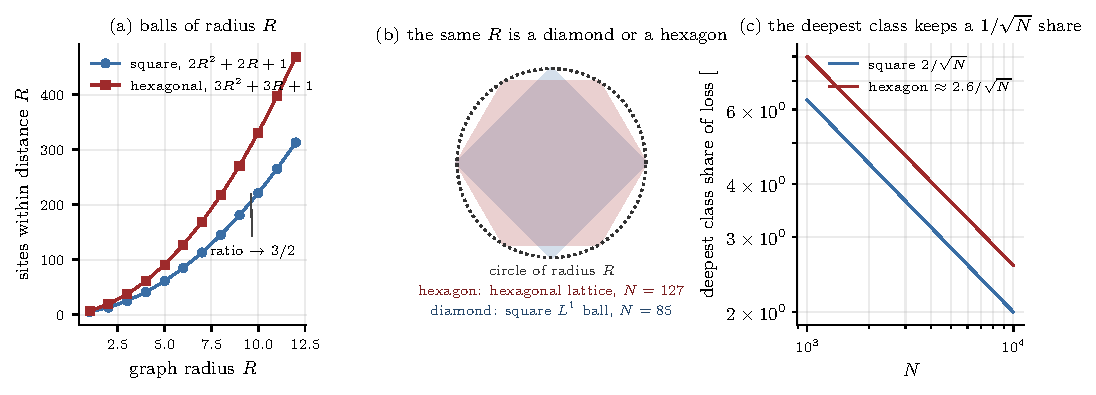
\includegraphics[width=0.76\linewidth]{figures/scaling.pdf}
\end{center}
\caption{Comparisons that follow from the two toppling matrices alone and involve no
avalanche measurement. (a) Sites within graph distance $R$: $2R^2+2R+1$ on the square
lattice against $3R^2+3R+1$ on the hexagonal one, a ratio approaching $3/2$. (b) The two
balls at $R = 6$: the square lattice's $L^1$ ball is a diamond and the hexagonal
lattice's is a hexagon, neither a circle. (c) The share of the total loss carried by the
deepest boundary class as $N \to \infty$: both fall off as $1/\sqrt{N}$, and the
hexagon's coefficient is $30\%$ larger.}
\label{fig:scaling}
\end{figure}

\section{Why the hexagonal grid is still Abelian}\label{sec:hexabelian}

Three reasons, in increasing order of generality.

\emph{The commutativity proof makes no use of the lattice.} Lemma~\ref{lem:commute} uses
exactly one fact about $\D$, namely $\D(\bm{x}_1,\bm{x}_2) \ge 0$ for
$\bm{x}_1 \neq \bm{x}_2$, which is \eqref{eq:4a}. It does not use the symmetry half of
\eqref{eq:4a}, the number of neighbours, the shape of the region, or planarity. The same
holds for Theorem~\ref{thm:abelianlemma}, where the only place the sign of an
off-diagonal entry enters is \eqref{eq:contradiction}, allowing $v_{t-1} \le w$ to be
pushed through the sum. Writing the critical step out for the hexagonal case, with
$\bm{x}_1,\bm{x}_2$ both unstable and distinct,
\begin{equation}\label{eq:hexcommute}
  \bigl(T_{\bm{x}_1}p\bigr)(\bm{x}_2) = p(\bm{x}_2) + \Dhex(\bm{x}_1,\bm{x}_2)
  \ \ge\ p(\bm{x}_2) \ \ge\ k_{\hx} ,
\end{equation}
so $\bm{x}_2$ is still unstable and the second toppling happens in either order. The
number $6$ appears nowhere in this line: it appears only in the diagonal entry, and the
diagonal entry does not enter the argument.

\emph{Termination and uniqueness transfer for the same reason.}
Proposition~\ref{prop:termination} and Theorem~\ref{thm:unique} rest on
\eqref{eq:4a}--\eqref{eq:4d} through the $M$-matrix property of $-\D$, which needs four
things of $-\D$: non-positive off-diagonal entries, strictly positive diagonal,
non-negative row sums with at least one strictly positive, and a connected off-diagonal
graph. On the hexagonal region these hold with the substitutions $4 \to 6$ and
``square'' $\to$ ``hexagon'': $-\Dhex(\bm{x},\bm{y}) = -1 \le 0$ for $\bm{x} \neq \bm{y}$;
$-\Dhex(\bm{x},\bm{x}) = 6 > 0$; row sums $6 - m(\bm{x}) \ge 0$ by \eqref{eq:rowsumhex},
strictly positive for each of the $6R$ boundary sites; and the off-diagonal pattern is
the adjacency of a connected graph. So $-\Dhex$ is again irreducibly diagonally dominant
and hence a nonsingular $M$-matrix, $\Dhex$ is invertible, and the firing vector
\begin{equation}\label{eq:firinghex}
  \sigma = \bigl(\Dhex^{-1}\bigr)^{\!\top}(p^\circ - p)
\end{equation}
is unique. Nothing in the argument refers to the lattice beyond those four properties,
each of which was checked in §\ref{sec:hextheta} directly from \eqref{eq:deltah}.

\emph{The general statement, which is the real reason.} The two arguments above are
instances of a fact stated at the right level of generality in the literature. Dhar
defines the Abelian sand pile on an arbitrary directed graph, with a toppling matrix
satisfying only the three sign conditions, and proves the Abelian property at that level
\cite{dhar1999}. Járai defines the same model on an arbitrary finite connected multigraph
$G = (V \cup \{s\}, E)$ with a sink, the stability threshold equal to the degree, and
$\D$ the graph Laplacian restricted to $V$, and proves that the stabilisation map is well
defined \cite{jarai2018}. In both formulations the lattice has already disappeared: it
enters only through the degrees and the adjacency, that is, through which entries of $\D$
are non-zero. The hexagonal lattice is therefore not a case needing a new proof but an
instance of the definition, and the correct statement is conditional: the stabilised
configuration is unique \emph{because $\Dhex$ is a graph Laplacian with non-positive row
sums, not because the neighbours happen to be six.}

This identifies what would break the property, and it is not the geometry. Two hypotheses
do the work: the instability test must involve the height of the site alone, and a
toppling must only add sand to other sites. The hexagonal lattice changes the value of
the diagonal entry and which pairs of sites are neighbours, but changes neither
hypothesis. Randomness is not by itself a failure either: the Manna model hands grains to
randomly chosen neighbours and is still Abelian, because the random rule is fixed per
site in advance \cite{manna1990,dhar1999}. Manna's model is Abelian and yet sits in a
different universality class, so Abelianity and shared exponents are independent
properties --- which is exactly the distinction
§\ref{sec:hexcompare} is built on.

\section{Comparison with the square baseline}\label{sec:hexcompare}

The comparison is clearest once the quantities are sorted into those supposed to be
universal and those not, because the prediction differs.

\begin{table}[htbp]
\centering
\small
\caption{The square baseline against the hexagonal extension. Quantities marked
\emph{universal} are predicted to agree; those marked \emph{lattice-specific} are
predicted to differ.}
\label{tab:hexcompare}
\begin{tabularx}{\textwidth}{l l l X}
\toprule
\textbf{Quantity} & \textbf{Square} & \textbf{Hexagonal} & \textbf{Status and reason} \\
\midrule
degree $z$ / threshold $k$ & $4$ & $6$
  & lattice-specific, forced by \eqref{eq:4c} \\[2pt]
row-sum classes & $\{0,-1,-2\}$ & $\{0,-2,-3\}$
  & lattice-specific, three classes each \\[2pt]
boundary sites & $4L-4$ & $6R$
  & lattice-specific; fraction $\approx 4/\sqrt{N}$ against $\approx 2\sqrt{3}/\sqrt{N}$ \\[2pt]
total dissipation & $4L$ & $12R+6$
  & lattice-specific; per boundary site $\to 1$ against $\to 2$ \\[2pt]
ball of radius $R$ & $2R^2+2R+1$ & $3R^2+3R+1$
  & ratio $\to 3/2$ \\[2pt]
length metric & $L^1$ & \eqref{eq:hexdist}
  & must change with the geometry \\[2pt]
mean height $\meanh$ & $17/8 = 2.125$ & $(5+\loopc_{\hx})/2$
  & lattice-specific; see below \\[2pt]
toppling exponent $\tau_s$ & $6/5$ & $6/5$
  & universal; see below \\[2pt]
area exponent $\tau_d$ & $5/4$ & $5/4$
  & universal; same \\[2pt]
group order $\absR$ & $\mathrm{e}^{\,4G N/\pi + o(N)}$ & $\mathrm{e}^{\,1.62 N + o(N)}$
  & lattice-specific; see below \\
\bottomrule
\end{tabularx}
\end{table}

\subsection{The exponents are predicted to stay the same}\label{sec:hexuniversal}

The avalanche exponents are not obtained by fitting them. They follow from an
equivalence: the recurrent configurations of the undirected sand pile are in bijection
with the spanning trees of the associated graph, and the spanning-tree model is the
$q \to 0$ limit of the $q$-state Potts model \cite{majumdar1992,dhar1999}. In two
dimensions that limit is a conformal field theory with central charge $c = -2$, and
exponents read off from it depend on $c$, hence on the dimension, and not on the lattice.
The chemical-path dimension of spanning trees is $5/4$, giving
$(\tau_t - 1) = \tfrac45(\tau_r - 1)$, and the wave decomposition of an avalanche leads to
the conjectured exact values
\begin{equation}\label{eq:tauexact}
  \tau_d = \frac54, \qquad \tau_s = \frac65, \qquad \tau_t = \frac75
\end{equation}
for distinct sites, topplings and duration, in the probability-density convention
\cite{dhar1999}. Because the derivation routes through a two-dimensional conformal field
theory and never through the square lattice, the exponents should be the same on the
hexagonal lattice: changing the degree from $4$ to $6$ changes the microscopic
coordination, not the dimension.

This is the main falsifiable prediction of the extension. The criterion is fixed in
advance: fit $\tau_s$ and $\tau_d$ on the hexagonal lattice at several sizes and require
the value to be stable in $N$ and consistent with $6/5$ and $5/4$ within the fitting
error. A deviation that does not shrink as $N$ grows would indicate that the degree
affects the effective conservation structure. One caution applies to the comparison. The
conjectured values are asymptotic, and a finite board returns a number above them because
of the cut-off of §\ref{sec:distributions}, so the comparison must be between two
lattices at the \emph{same} sizes with the \emph{same} procedure, never between a fitted
and a theoretical number; and since the cut-off sits at a different place on the two
lattices, the size dependence is checked before the exponents are compared.

\subsection{The mean height is predicted to change}\label{sec:hexmeanh}

The mean height is not universal, and the square baseline's exact value says how and why.
On a $z$-regular lattice the mean height and the looping constant are related by
\begin{equation}\label{eq:zetaxi}
  \meanh = \frac{z - 1 + \loopc}{2},
  \qquad
  \loopc = \mathbb{E}\bigl[\#\{\text{neighbours of } o
        \text{ visited by the infinite LERW from } o\}\bigr] ,
\end{equation}
where the loop-erased random walk is obtained by erasing loops from a simple random walk
as they are created, and the relation is derived from the burning bijection in
\cite{jarai2018}, §5.5.2; see also \cite{kassel2016} for the looping rate of planar
graphs.

The relation explains the square lattice's exact value as a special case. On
$\mathbb{Z}^2$ the looping constant is $\loopc = 5/4$, proved in
\cite{poghosyan2011,levine2014}, so
\begin{equation}\label{eq:zetasq}
  \meanh_{\sq} = \frac{4 - 1 + 5/4}{2} = \frac{17}{8} = 2.125 ,
\end{equation}
reproducing \eqref{eq:meanh} by a different route. It gives the hexagonal prediction in
closed form,
\begin{equation}\label{eq:zetahex}
  \meanh_{\hx} = \frac{6 - 1 + \loopc_{\hx}}{2} = \frac{5 + \loopc_{\hx}}{2} ,
\end{equation}
where $\loopc_{\hx}$ is the looping constant of the triangular lattice, and it shows that
$\meanh_{\hx}$ is \emph{not} obtained by rescaling $17/8$ by the threshold ratio. That
argument gives $2.125 \times 6/4 = 3.1875$, which by \eqref{eq:zetahex} would require
$\loopc_{\hx} = 1.375$, while keeping $\loopc = 1.25$ gives $3.125$; the two differ
because \eqref{eq:zetaxi} does not fix $\loopc_{\hx}$, and no derivation selects one. The
relation does give a bound and a target: since $1 \le \loopc_{\hx} \le 6$ trivially,
$\meanh_{\hx} \in [3, 5.5]$, and a range comparable to $\loopc = 1.25$ narrows this to
roughly $[3.1, 3.6]$. It also makes the measurement a sharp one, since measuring
$\meanh_{\hx}$ to four decimals determines $\loopc_{\hx}$ to four decimals. On the square
lattice the same measurement can be checked against a theorem, because $5/4$ is proved;
for the triangular lattice no closed form is used here, and the measured value stands on
its own.

\subsection{The algebraic complexity changes, without affecting universality}
\label{sec:hexgroup}

One further quantity is neither a statistic nor an exponent. The number of recurrent
configurations is the sand pile group order, $\absR = \det(-\D)$ of
\eqref{eq:recurrentcount}, also the number of spanning trees of the wired graph obtained
by attaching a sink to every off-board direction \cite{dhar1999,klivans2019}. It grows
exponentially in $N$, so the interesting number is the spanning-tree entropy per site,
$h = \lim_{N\to\infty} \frac1N \log \absR$. On the square lattice this limit is the
classical $4G/\pi = 1.16624$, with $G$ Catalan's constant \cite{lyons2005}; on the
hexagonal lattice it must be larger, since each site has more neighbours. Extrapolating
$\frac1N\log\det(-\D)$ in $1/R$ gives $h_{\hx} \approx 1.62$, about $39\%$ above the
square value, and the same extrapolation on the square lattice returns $1.1672$ against
the exact $1.16624$, an error of $9\times10^{-4}$ --- which is what makes the hexagonal
number worth quoting to two decimals and no more. Two lattices can therefore share every
avalanche exponent and still have sand pile groups of different exponential size:
universality is a statement about the statistics, not the algebra, and if $\tau_s$
agrees with the baseline as predicted the group order will still differ by a factor
$e^{(1.62-1.166)N}$.

\section{What is to be measured}\label{sec:hexplan}

The program changes in two places only: the toppling rule uses the six directions
\eqref{eq:hexdirs}, and the length observable uses \eqref{eq:hexdist}. The board is still
a one-dimensional array of length $N_{\hx}$, a record is still four integers, and the
main loop of §\ref{sec:storage} is untouched. That the main loop does not move is itself
the check that the geometry was separated properly: the lattice is a parameter object
satisfying the \texttt{TopplingMatrix} concept of Appendix~\ref{app:sigs}, so a new
lattice is a new class and not a new simulation. Every quantity below is to be measured
with the same seeds, burn-in and fitting code as the baseline, and the board size
reported alongside each number, since both the exponent and the cut-off $s_\xi \sim L^D$
depend on it.

\begin{table}[htbp]
\centering
\small
\caption{Quantities to be measured on the hexagonal lattice, with the expected value and
the criterion that would count as a disagreement.}
\label{tab:hexplan}
\begin{tabularx}{\textwidth}{l l X}
\toprule
\textbf{Quantity} & \textbf{Expected} & \textbf{Test and criterion} \\
\midrule
threshold $k_{\hx}$ & $6$
  & read from $-\Dhex(\bm{x},\bm{x})$; a different value would mean \eqref{eq:4c} fails \\[2pt]
mean height $\meanh_{\hx}$ & $(5+\loopc_{\hx})/2$
  & average after $2N$ burn-in; the measured value determines $\loopc_{\hx}$ \\[2pt]
loss rate $\bar{l}$ & $1$
  & grains lost per drop; input--output balance, must hold on both lattices \\[2pt]
topples $\tau_s$, area $\tau_d$ & $6/5$ and $5/4$
  & MLE at a common $x_{\min}$ and common $N$; agreement within fitting error accepts one
    universality class, a size-stable deviation reports new exponents \\[2pt]
length $\tau_R$, $E[l\mid R]$, $D$ & metric-dependent
  & measure $\tau_R$ with \eqref{eq:hexdist}; bin $E[l\mid R]$ to expose the corner; at
    least three sizes, and if the $s/N^{D}$ curves do not overlap adjust $D$ first \\[2pt]
boundary row sums & $\{0,-2,-3\}$
  & recomputed from $\Dhex$; a value of $-1$ would mean the region is not a hexagon \\[2pt]
Abelian property & holds
  & stabilise one configuration by queue, stack and random order; the firing vectors must
    agree exactly \\
\bottomrule
\end{tabularx}
\end{table}

\begin{pending}
  \pendingtag The measurements of Table~\ref{tab:hexplan} have not been carried out. The
  implementation still to be added is a second class satisfying the
  \texttt{TopplingMatrix} concept, with the directions \eqref{eq:hexdirs} and the metric
  \eqref{eq:hexdist}; after that the simulation is a recompilation of the existing code.
  The order of work is: first the square-lattice runs of §\ref{sec:burnin}, long enough
  to fix $\tau_s$ and $\tau_d$ on the baseline; then the same runs on the hexagonal
  lattice at matched sizes; and finally the collapse across sizes, with $D$ adjusted
  before any exponent is reinterpreted. The criterion for accepting a single universality
  class is stated with the exponents above.
\end{pending}
